\section{Battery \& battery holder}
The purpose of this block is to deliver electrical energy to supply the  Propulsion Motor as well as the accessory systems in the car.

\subsection{Analysis}
This unit consists of twelve battery cells, which are responsible for storing electrical energy. Moreover, it must be capable of delivering the required current to turn the propulsion motor and be able to acquire energy from an external charger.   
The requirements for batteries when participating in the SEM are that the prototype battery electric class must utilize lithium type batteries. There was two choices between lithium type batteries: LiFePo4 and Lithium-ion polymer(Li-Po). Based on the tests done by Jonas \fxnote{REFERENCE to BMS "see Battery cell type test.pdf"} the Li-Po is the obvious choice, since it has a more satisfying capacity at the simulated worst case Eco-Marathon conditions. Moreover, it has a solid low internal resistance and weight for the purpose.\\
Since the Li-Po batteries are the better choice compared to the LiFePo4 batteries there will be used two Li-Po batteries in series to power the vehicle. Each of the batteries will have 6 cells, which results in a nominal voltage of 44.4V since each cell's nominal voltage is 3.7V. By doing so we are still within our limitations of having the voltage to not exceed the maximum of 48V nominal as specified by AU2\_NF3. See section: \ref{sec:requirements}.\\
The batteries which have been purchased are of different capacities, however, they all have the same amount of cells, thus the same nominal voltage. This is done in preparation to test the required capacity needed by the vehicle. Furthermore, to be able to have a battery which weighs less if the given capacity is more than enough for a run will improve the effectiveness of the car, since the motor will have less weight to pull.\\

\begin{figure}[H]
	\centering
	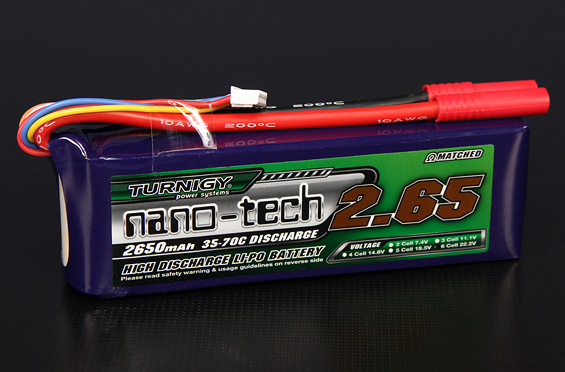
\includegraphics[width=0.6\linewidth]{Hardware/Pictures/2650battery}
	\caption[Empty]{Picture of the battery with 2650mAh\footnotemark}
	\label{fig:2650battery}
\end{figure}
\footnotetext{\url{http://www.hobbyking.com/hobbyking/store/__32651__Turnigy_nano_tech_2650mAh_6S_35_70C_Lipo_Pack_EU_Warehouse_.html} (Date: 20-05-2016)}

\textbf{Battery specifications}\\
Chemistry: Lithium-ion polymer(Li-cobalt)\\
Manufacturer: Turnigy\\
Type: Nano-tech\\
Nominal: 44.4V\\
Max. charging voltage: 50.4V\\
Min. voltage: 36V\\
Capacity: 2200 / 2650 / 3300mAh (depends on weather and achieved efficiency)\\
Max. continuous discharge: 35 / 35 / 45C\\
Max. charge rate: 8 / 8 / 10C\\
Weight: 730 / 834 / 1130g\\


\subsection{Implementation}
text

\subsection{Unity test}
text